\begin{enumerate}[label=\thechapter.\arabic*,ref=\thechapter.\theenumi]

\item In a potato race, a bucket is placed at the starting point, which is 5 m from the first potato,and the other potatoes are placed 3 m apart in a straight line. There are ten potatoes in the line. A competitor starts from the bucket, picks up the nearest potato, runs back with it, drops it in the bucket, runs back to pick up the next potato, runs to the bucket to drop it in, and she continues in the same way until all the potatoes are in the bucket. What is the total distance the competitor has to run?\\
\hfill(NCERT-Maths 10.5.3.20Q)\\
\solution 
 \iffalse
\let\negmedspace\undefined
\let\negthickspace\undefined
\documentclass[journal,12pt,twocolumn]{IEEEtran}
\usepackage{amssymb}
\usepackage{cite}
\usepackage{amsmath,amssymb,amsfonts,amsthm}
\usepackage{algorithmic}
\usepackage{graphicx}
\usepackage{textcomp}
\usepackage{xcolor}
\usepackage{txfonts}
\usepackage{listings}
\usepackage{enumitem}
\usepackage{mathtools}
\usepackage{gensymb}
\usepackage{comment}
\usepackage[breaklinks=true]{hyperref}
\usepackage{tkz-euclide} 
\usepackage{listings}
\usepackage{gvv}                                        
\def\inputGnumericTable{}                                 
\usepackage[latin1]{inputenc}                                
\usepackage{color}                                            
\usepackage{array}                                            
\usepackage{longtable}                                       
\usepackage{calc}                                             
\usepackage{multirow}                                         
\usepackage{hhline}                                           
\usepackage{ifthen}                                           
\usepackage{lscape}
\usepackage{pgfplots}
\newtheorem{theorem}{Theorem}[section]
\newtheorem{problem}{Problem}
\newtheorem{proposition}{Proposition}[section]
\newtheorem{lemma}{Lemma}[section]
\newtheorem{corollary}[theorem]{Corollary}
\newtheorem{example}{Example}[section]
\newtheorem{definition}[problem]{Definition}
\newcommand{\BEQA}{\begin{eqnarray}}
\newcommand{\EEQA}{\end{eqnarray}}
\newcommand{\define}{\stackrel{\triangle}{=}}
\theoremstyle{remark}
\newtheorem{rem}{Remark}
\begin{document}

\bibliographystyle{IEEEtran}
\vspace{3cm}

\title{NCERT Discrete-11.9.4-5}
\author{EE22BTECH11004 - Allu Lohith}

\maketitle
\newpage
\bigskip


 Find the sum of n terms of this sequence:$$5^2+6^2+7^2...+20^2$$  
\solution
\fi
\begin{table}[h!]
\centering
\renewcommand{\arraystretch}{2}
\begin{tabular}{|c|p{4cm}|c|}
\hline 
\setlength{\tabcolsep}{1pt}
\textbf{Parameter}  &\textbf{Description} &\textbf{Formulae/Value} \\
\hline
n & Iteration number starting from zero till 15 & - \\
\hline
$x\brak n$ & General term of the sequence from $n=0$ to $n=15$ &$\brak{n+5}^2$  u\brak n\\
\hline
$x\brak 0$ & First term of the sequence & 5 \\
\hline
\end{tabular}

\vspace{0.5cm}
\caption{\normalsize Parameters}
\end{table}
The standard $z$ transforms,
\begin{align}
    u \brak n &\stackrel{z}{\longleftrightarrow} \frac{1}{1-z^{-1}}, \abs z >1\\
   n u\brak n &\stackrel{z}{\longleftrightarrow} \frac{z^{-1}}{\brak{1-z^{-1}}^2}, \abs z >1\\
   n^2 u\brak n &\stackrel{z}{\longleftrightarrow} \frac{z^{-1}\brak{1+z^{-1}}}{\brak{1-z^{-1}}^3}, \abs z >1
\end{align}
As 
\begin{align}
    x\brak n = \brak{n^2+10n+25}u\brak n
\end{align}
The $z$ transform of general term can be written as , 
\begin{align}
    X\brak z &= \frac{z^{-1}\brak{1+z^{-1}}}{\brak{1-z^{-1}}^3}+10\frac{z^{-1}}{\brak{1-z^{-1}}^2}+\frac{25}{1-z^{-1}} \\
    X\brak z &=  \frac{16z^{-2}-39z^{-1}+25}{\brak{1-z^{-1}}^3}; \abs{z}>1
\end{align}
On convolution for finding the sum
\begin{align}
    y\brak n= x\brak n \ast u\brak n
\end{align}
On z transform,
\begin{align}
    Y\brak z &= X \brak z \cdot U \brak z\\
    &= \brak{\frac{16z^{-2}-39z^{-1}+25}{\brak{1-z^{-1}})^3}} \cdot \frac{1}{1-z^{-1}}\\
    \implies 
    Y \brak z & = \frac{16z^{-2}-39z^{-1}+25}{\brak{1-z^{-1}}^4}; \quad \abs z >1
\end{align}
Using the contour integration to find the inverse $z$ transform,
\begin{align}
    y(n)&=\oint_c Y(z)\cdot z^{n-1}dz\\
    y(21)&=\oint_c \brak{\frac{16z^{-2}-39z^{-1}+25}{\brak{1-z^{-1}}^4}} z^{14}dz
\end{align}
As there are four poles from observation, so $m=4$
\begin{align}
    y\brak{21} &= \frac{1}{(m-1)!} \lim_{z \to a} \frac{d^{m-1}}{dz^{m-1}}\brak{(z-a)^mf(z)}\\
    &= \frac{1}{3!} \lim_{z \to 1} \frac{d^{3}}{dz^{3}}\brak{(z-1)^4 \frac{\brak{16z^{-2}-39z^{-1}+25}}{(1-z^{-1})^4} z^{14}}\\
    &= \frac{1}{6} \lim_{z \to 1} \frac{d^{3}}{dz^{3}}\brak{\brak{16z^{-2}-39z^{-1}+25}z^{18}}\\
    &= \frac{1}{6} \lim_{z \to 1} \frac{d^{3}}{dz^{3}}\brak{16z^{16}-39z^{17}+25z^{18}}\\
    &= \frac{1}{6}  \brak{16 \times 18 \times 17 \times 16+14 \times 17 \times 16 \times 15 }\\
    \implies y\brak{21}&=2840 
\end{align}
Hence the sum of the terms of the sequence is 2840.

\begin{figure}[h]
    \centering  

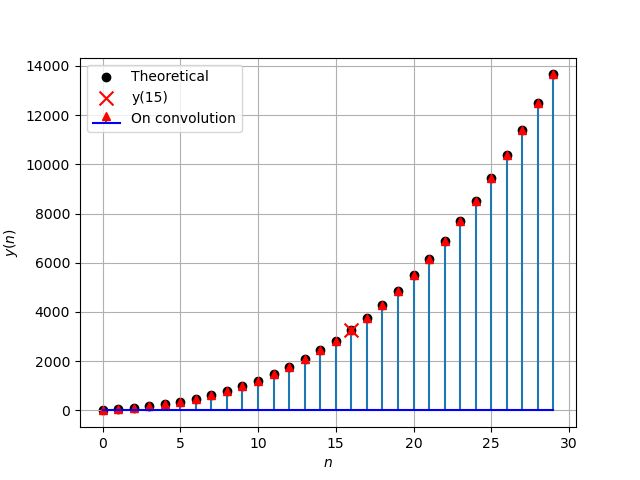
\includegraphics[width=\columnwidth]{ncert-maths/11/9/4/5/figs/plot.png}

\begin{center}
    \caption{Simulation v/s theoretical}
\end{center}
\end{figure}


\pagebreak

\item Find the sum of the first $15$ multiples of $8$. \\

\solution
\input{ncert-maths/10/5/3/13/assignment12.tex}
ss\pagebreak

\item If the sum of $n$ terms of an A.P. is $3n^2+5n$ and its $m^{th}$ term is 164, find the value of $m$.\\
\solution
 \iffalse
\let\negmedspace\undefined
\let\negthickspace\undefined
\documentclass[journal,12pt,twocolumn]{IEEEtran}
\usepackage{amssymb}
\usepackage{cite}
\usepackage{amsmath,amssymb,amsfonts,amsthm}
\usepackage{algorithmic}
\usepackage{graphicx}
\usepackage{textcomp}
\usepackage{xcolor}
\usepackage{txfonts}
\usepackage{listings}
\usepackage{enumitem}
\usepackage{mathtools}
\usepackage{gensymb}
\usepackage{comment}
\usepackage[breaklinks=true]{hyperref}
\usepackage{tkz-euclide} 
\usepackage{listings}
\usepackage{gvv}                                        
\def\inputGnumericTable{}                                 
\usepackage[latin1]{inputenc}                                
\usepackage{color}                                            
\usepackage{array}                                            
\usepackage{longtable}                                       
\usepackage{calc}                                             
\usepackage{multirow}                                         
\usepackage{hhline}                                           
\usepackage{ifthen}                                           
\usepackage{lscape}
\usepackage{pgfplots}
\newtheorem{theorem}{Theorem}[section]
\newtheorem{problem}{Problem}
\newtheorem{proposition}{Proposition}[section]
\newtheorem{lemma}{Lemma}[section]
\newtheorem{corollary}[theorem]{Corollary}
\newtheorem{example}{Example}[section]
\newtheorem{definition}[problem]{Definition}
\newcommand{\BEQA}{\begin{eqnarray}}
\newcommand{\EEQA}{\end{eqnarray}}
\newcommand{\define}{\stackrel{\triangle}{=}}
\theoremstyle{remark}
\newtheorem{rem}{Remark}
\begin{document}

\bibliographystyle{IEEEtran}
\vspace{3cm}

\title{NCERT Discrete-11.9.4-5}
\author{EE22BTECH11004 - Allu Lohith}

\maketitle
\newpage
\bigskip


 Find the sum of n terms of this sequence:$$5^2+6^2+7^2...+20^2$$  
\solution
\fi
\begin{table}[h!]
\centering
\renewcommand{\arraystretch}{2}
\begin{tabular}{|c|p{4cm}|c|}
\hline 
\setlength{\tabcolsep}{1pt}
\textbf{Parameter}  &\textbf{Description} &\textbf{Formulae/Value} \\
\hline
n & Iteration number starting from zero till 15 & - \\
\hline
$x\brak n$ & General term of the sequence from $n=0$ to $n=15$ &$\brak{n+5}^2$  u\brak n\\
\hline
$x\brak 0$ & First term of the sequence & 5 \\
\hline
\end{tabular}

\vspace{0.5cm}
\caption{\normalsize Parameters}
\end{table}
The standard $z$ transforms,
\begin{align}
    u \brak n &\stackrel{z}{\longleftrightarrow} \frac{1}{1-z^{-1}}, \abs z >1\\
   n u\brak n &\stackrel{z}{\longleftrightarrow} \frac{z^{-1}}{\brak{1-z^{-1}}^2}, \abs z >1\\
   n^2 u\brak n &\stackrel{z}{\longleftrightarrow} \frac{z^{-1}\brak{1+z^{-1}}}{\brak{1-z^{-1}}^3}, \abs z >1
\end{align}
As 
\begin{align}
    x\brak n = \brak{n^2+10n+25}u\brak n
\end{align}
The $z$ transform of general term can be written as , 
\begin{align}
    X\brak z &= \frac{z^{-1}\brak{1+z^{-1}}}{\brak{1-z^{-1}}^3}+10\frac{z^{-1}}{\brak{1-z^{-1}}^2}+\frac{25}{1-z^{-1}} \\
    X\brak z &=  \frac{16z^{-2}-39z^{-1}+25}{\brak{1-z^{-1}}^3}; \abs{z}>1
\end{align}
On convolution for finding the sum
\begin{align}
    y\brak n= x\brak n \ast u\brak n
\end{align}
On z transform,
\begin{align}
    Y\brak z &= X \brak z \cdot U \brak z\\
    &= \brak{\frac{16z^{-2}-39z^{-1}+25}{\brak{1-z^{-1}})^3}} \cdot \frac{1}{1-z^{-1}}\\
    \implies 
    Y \brak z & = \frac{16z^{-2}-39z^{-1}+25}{\brak{1-z^{-1}}^4}; \quad \abs z >1
\end{align}
Using the contour integration to find the inverse $z$ transform,
\begin{align}
    y(n)&=\oint_c Y(z)\cdot z^{n-1}dz\\
    y(21)&=\oint_c \brak{\frac{16z^{-2}-39z^{-1}+25}{\brak{1-z^{-1}}^4}} z^{14}dz
\end{align}
As there are four poles from observation, so $m=4$
\begin{align}
    y\brak{21} &= \frac{1}{(m-1)!} \lim_{z \to a} \frac{d^{m-1}}{dz^{m-1}}\brak{(z-a)^mf(z)}\\
    &= \frac{1}{3!} \lim_{z \to 1} \frac{d^{3}}{dz^{3}}\brak{(z-1)^4 \frac{\brak{16z^{-2}-39z^{-1}+25}}{(1-z^{-1})^4} z^{14}}\\
    &= \frac{1}{6} \lim_{z \to 1} \frac{d^{3}}{dz^{3}}\brak{\brak{16z^{-2}-39z^{-1}+25}z^{18}}\\
    &= \frac{1}{6} \lim_{z \to 1} \frac{d^{3}}{dz^{3}}\brak{16z^{16}-39z^{17}+25z^{18}}\\
    &= \frac{1}{6}  \brak{16 \times 18 \times 17 \times 16+14 \times 17 \times 16 \times 15 }\\
    \implies y\brak{21}&=2840 
\end{align}
Hence the sum of the terms of the sequence is 2840.

\begin{figure}[h]
    \centering  

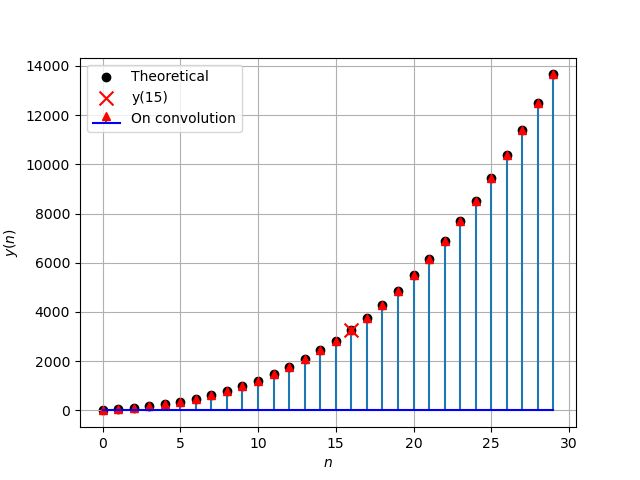
\includegraphics[width=\columnwidth]{ncert-maths/11/9/4/5/figs/plot.png}

\begin{center}
    \caption{Simulation v/s theoretical}
\end{center}
\end{figure}



\pagebreak
\item Find the sums given below:
\begin{enumerate}
    \item  $7 + \frac{21}{2} + 14 ... + 84$
    \item  $34 + 32 + 30 ... + 10$
    \item  $-5 + -8 + -11 ... -230$
\end{enumerate}
\solution
\input{ncert-maths/10/5/3/2/a1.tex}
\pagebreak
\item Show that $a_0$ , $a_1$ , $a_2$
, . . ., $a_n$
, . . . form an AP where an is defined as below :
\begin{enumerate}
    \item $a_n$ = $(3 + 4n)$ 
    \item $a_n$ = $(9 - 5n)$ 
\end{enumerate}
Also find the sum of the first 15 terms in each case.
\solution
\input{ncert-maths/10/5/3/10/math.10.5.3.10.tex}

\pagebreak
\item If the sum of $n$ terms of an AP is $(pn + qn^2)$, where $p$ and $q$ are constants, find the common difference.
\solution
		\input{ncert-maths/11/9/2/8/Math_11_9_2_8.tex}

\pagebreak
\item Find the sum of the first 40 positive integers divisible by 6\\
	\solution
		 \iffalse
\let\negmedspace\undefined
\let\negthickspace\undefined
\documentclass[journal,12pt,twocolumn]{IEEEtran}
\usepackage{amssymb}
\usepackage{cite}
\usepackage{amsmath,amssymb,amsfonts,amsthm}
\usepackage{algorithmic}
\usepackage{graphicx}
\usepackage{textcomp}
\usepackage{xcolor}
\usepackage{txfonts}
\usepackage{listings}
\usepackage{enumitem}
\usepackage{mathtools}
\usepackage{gensymb}
\usepackage{comment}
\usepackage[breaklinks=true]{hyperref}
\usepackage{tkz-euclide} 
\usepackage{listings}
\usepackage{gvv}                                        
\def\inputGnumericTable{}                                 
\usepackage[latin1]{inputenc}                                
\usepackage{color}                                            
\usepackage{array}                                            
\usepackage{longtable}                                       
\usepackage{calc}                                             
\usepackage{multirow}                                         
\usepackage{hhline}                                           
\usepackage{ifthen}                                           
\usepackage{lscape}
\usepackage{pgfplots}
\newtheorem{theorem}{Theorem}[section]
\newtheorem{problem}{Problem}
\newtheorem{proposition}{Proposition}[section]
\newtheorem{lemma}{Lemma}[section]
\newtheorem{corollary}[theorem]{Corollary}
\newtheorem{example}{Example}[section]
\newtheorem{definition}[problem]{Definition}
\newcommand{\BEQA}{\begin{eqnarray}}
\newcommand{\EEQA}{\end{eqnarray}}
\newcommand{\define}{\stackrel{\triangle}{=}}
\theoremstyle{remark}
\newtheorem{rem}{Remark}
\begin{document}

\bibliographystyle{IEEEtran}
\vspace{3cm}

\title{NCERT Discrete-11.9.4-5}
\author{EE22BTECH11004 - Allu Lohith}

\maketitle
\newpage
\bigskip


 Find the sum of n terms of this sequence:$$5^2+6^2+7^2...+20^2$$  
\solution
\fi
\begin{table}[h!]
\centering
\renewcommand{\arraystretch}{2}
\begin{tabular}{|c|p{4cm}|c|}
\hline 
\setlength{\tabcolsep}{1pt}
\textbf{Parameter}  &\textbf{Description} &\textbf{Formulae/Value} \\
\hline
n & Iteration number starting from zero till 15 & - \\
\hline
$x\brak n$ & General term of the sequence from $n=0$ to $n=15$ &$\brak{n+5}^2$  u\brak n\\
\hline
$x\brak 0$ & First term of the sequence & 5 \\
\hline
\end{tabular}

\vspace{0.5cm}
\caption{\normalsize Parameters}
\end{table}
The standard $z$ transforms,
\begin{align}
    u \brak n &\stackrel{z}{\longleftrightarrow} \frac{1}{1-z^{-1}}, \abs z >1\\
   n u\brak n &\stackrel{z}{\longleftrightarrow} \frac{z^{-1}}{\brak{1-z^{-1}}^2}, \abs z >1\\
   n^2 u\brak n &\stackrel{z}{\longleftrightarrow} \frac{z^{-1}\brak{1+z^{-1}}}{\brak{1-z^{-1}}^3}, \abs z >1
\end{align}
As 
\begin{align}
    x\brak n = \brak{n^2+10n+25}u\brak n
\end{align}
The $z$ transform of general term can be written as , 
\begin{align}
    X\brak z &= \frac{z^{-1}\brak{1+z^{-1}}}{\brak{1-z^{-1}}^3}+10\frac{z^{-1}}{\brak{1-z^{-1}}^2}+\frac{25}{1-z^{-1}} \\
    X\brak z &=  \frac{16z^{-2}-39z^{-1}+25}{\brak{1-z^{-1}}^3}; \abs{z}>1
\end{align}
On convolution for finding the sum
\begin{align}
    y\brak n= x\brak n \ast u\brak n
\end{align}
On z transform,
\begin{align}
    Y\brak z &= X \brak z \cdot U \brak z\\
    &= \brak{\frac{16z^{-2}-39z^{-1}+25}{\brak{1-z^{-1}})^3}} \cdot \frac{1}{1-z^{-1}}\\
    \implies 
    Y \brak z & = \frac{16z^{-2}-39z^{-1}+25}{\brak{1-z^{-1}}^4}; \quad \abs z >1
\end{align}
Using the contour integration to find the inverse $z$ transform,
\begin{align}
    y(n)&=\oint_c Y(z)\cdot z^{n-1}dz\\
    y(21)&=\oint_c \brak{\frac{16z^{-2}-39z^{-1}+25}{\brak{1-z^{-1}}^4}} z^{14}dz
\end{align}
As there are four poles from observation, so $m=4$
\begin{align}
    y\brak{21} &= \frac{1}{(m-1)!} \lim_{z \to a} \frac{d^{m-1}}{dz^{m-1}}\brak{(z-a)^mf(z)}\\
    &= \frac{1}{3!} \lim_{z \to 1} \frac{d^{3}}{dz^{3}}\brak{(z-1)^4 \frac{\brak{16z^{-2}-39z^{-1}+25}}{(1-z^{-1})^4} z^{14}}\\
    &= \frac{1}{6} \lim_{z \to 1} \frac{d^{3}}{dz^{3}}\brak{\brak{16z^{-2}-39z^{-1}+25}z^{18}}\\
    &= \frac{1}{6} \lim_{z \to 1} \frac{d^{3}}{dz^{3}}\brak{16z^{16}-39z^{17}+25z^{18}}\\
    &= \frac{1}{6}  \brak{16 \times 18 \times 17 \times 16+14 \times 17 \times 16 \times 15 }\\
    \implies y\brak{21}&=2840 
\end{align}
Hence the sum of the terms of the sequence is 2840.

\begin{figure}[h]
    \centering  

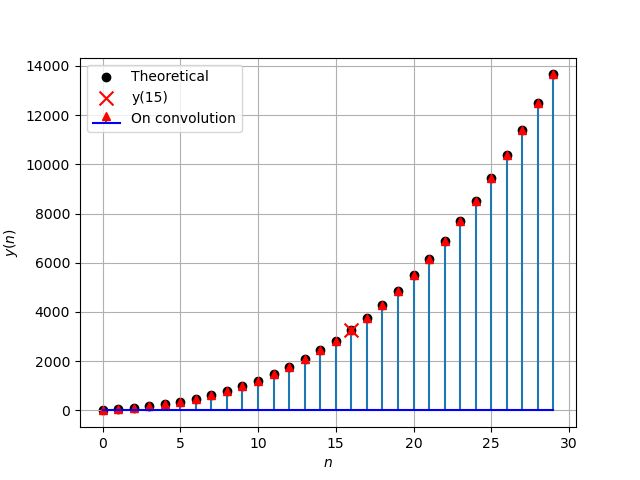
\includegraphics[width=\columnwidth]{ncert-maths/11/9/4/5/figs/plot.png}

\begin{center}
    \caption{Simulation v/s theoretical}
\end{center}
\end{figure}


\pagebreak
\item If the sum of certain number of terms in a AP 25,22,19,... is 116. Find the last term.\\
\solution
\input{ncert-maths/11/9/2/6/2.tex}
\pagebreak

\item The first and the last terms of an AP are 17 and 350 respectively. If the common difference
is 9, how many terms are there and what is their sum?\\
\solution 
\input{ncert-maths/10/5/3/6/10.5.3.tex}
\pagebreak
\item A small terrace at a football ground comprises of 15 steps each of which is 50
m long and built of solid concrete.Each step has a rise of 1/4 m and a tread of
1/2 m. Calculate the total volume of concrete required to build the terrace.
[Hint: Volume of concrete required to build the first step=\begin{align}
    V&=\frac{1}{4} \cdot \frac{1}{2} \cdot 50 
\end{align}\\
\solution 
\input{ncert-maths/10/5/4/5/assign1.tex}
\pagebreak

\item Given a GP with a = 729 and $7^{th}$ term 64, find $S_7$.\\
\solution 
\input{ncert-maths/11/9/3/15/ncert_11_9_3_15.tex}
\pagebreak

\item Find the sum of all natural numbers lying between 100 and 1000, which are
multiples of 5.\\
\solution
\input{ncert-maths/11/9/2/2/2.tex}
\pagebreak

\item Find the sum of odd numbers between 0 and 50.\\
\solution
\input{ncert-maths/10/5/3/14/14.tex}
\pagebreak

\item  A ladder has rungs 25cm apart.The rungs decrease uniformly in length from 45cm at the bottom to 25cm at the top.If the top and bottom rungs are 2 and 1/2 meter apart.what is length of wood required for the rungs?\\
\solution
\input{ncert-maths/10/5/4/3/second.tex}
\pagebreak

\item Q2) The sum of the third and the seventh terms of AP is 6 and their product is 8. Find the sum of first sixteen terms of the AP \\
\solution \input{ncert-maths/10/5/4/2/latexcode,discrete_pr.tex}
\pagebreak
\item A spiral is made up of successive semicircles, with centres alternately at A and B, starting with centre at A, of radii $0.5 cm$, $1.0 cm$, $1.5 cm$, $2.0 cm$, . . . What is the total length of such a spiral made up of thirteen consecutive semicircles? (Take $\pi = \frac{22}{7}$)\\
\solution
 \iffalse
\let\negmedspace\undefined
\let\negthickspace\undefined
\documentclass[journal,12pt,twocolumn]{IEEEtran}
\usepackage{amssymb}
\usepackage{cite}
\usepackage{amsmath,amssymb,amsfonts,amsthm}
\usepackage{algorithmic}
\usepackage{graphicx}
\usepackage{textcomp}
\usepackage{xcolor}
\usepackage{txfonts}
\usepackage{listings}
\usepackage{enumitem}
\usepackage{mathtools}
\usepackage{gensymb}
\usepackage{comment}
\usepackage[breaklinks=true]{hyperref}
\usepackage{tkz-euclide} 
\usepackage{listings}
\usepackage{gvv}                                        
\def\inputGnumericTable{}                                 
\usepackage[latin1]{inputenc}                                
\usepackage{color}                                            
\usepackage{array}                                            
\usepackage{longtable}                                       
\usepackage{calc}                                             
\usepackage{multirow}                                         
\usepackage{hhline}                                           
\usepackage{ifthen}                                           
\usepackage{lscape}
\usepackage{pgfplots}
\newtheorem{theorem}{Theorem}[section]
\newtheorem{problem}{Problem}
\newtheorem{proposition}{Proposition}[section]
\newtheorem{lemma}{Lemma}[section]
\newtheorem{corollary}[theorem]{Corollary}
\newtheorem{example}{Example}[section]
\newtheorem{definition}[problem]{Definition}
\newcommand{\BEQA}{\begin{eqnarray}}
\newcommand{\EEQA}{\end{eqnarray}}
\newcommand{\define}{\stackrel{\triangle}{=}}
\theoremstyle{remark}
\newtheorem{rem}{Remark}
\begin{document}

\bibliographystyle{IEEEtran}
\vspace{3cm}

\title{NCERT Discrete-11.9.4-5}
\author{EE22BTECH11004 - Allu Lohith}

\maketitle
\newpage
\bigskip


 Find the sum of n terms of this sequence:$$5^2+6^2+7^2...+20^2$$  
\solution
\fi
\begin{table}[h!]
\centering
\renewcommand{\arraystretch}{2}
\begin{tabular}{|c|p{4cm}|c|}
\hline 
\setlength{\tabcolsep}{1pt}
\textbf{Parameter}  &\textbf{Description} &\textbf{Formulae/Value} \\
\hline
n & Iteration number starting from zero till 15 & - \\
\hline
$x\brak n$ & General term of the sequence from $n=0$ to $n=15$ &$\brak{n+5}^2$  u\brak n\\
\hline
$x\brak 0$ & First term of the sequence & 5 \\
\hline
\end{tabular}

\vspace{0.5cm}
\caption{\normalsize Parameters}
\end{table}
The standard $z$ transforms,
\begin{align}
    u \brak n &\stackrel{z}{\longleftrightarrow} \frac{1}{1-z^{-1}}, \abs z >1\\
   n u\brak n &\stackrel{z}{\longleftrightarrow} \frac{z^{-1}}{\brak{1-z^{-1}}^2}, \abs z >1\\
   n^2 u\brak n &\stackrel{z}{\longleftrightarrow} \frac{z^{-1}\brak{1+z^{-1}}}{\brak{1-z^{-1}}^3}, \abs z >1
\end{align}
As 
\begin{align}
    x\brak n = \brak{n^2+10n+25}u\brak n
\end{align}
The $z$ transform of general term can be written as , 
\begin{align}
    X\brak z &= \frac{z^{-1}\brak{1+z^{-1}}}{\brak{1-z^{-1}}^3}+10\frac{z^{-1}}{\brak{1-z^{-1}}^2}+\frac{25}{1-z^{-1}} \\
    X\brak z &=  \frac{16z^{-2}-39z^{-1}+25}{\brak{1-z^{-1}}^3}; \abs{z}>1
\end{align}
On convolution for finding the sum
\begin{align}
    y\brak n= x\brak n \ast u\brak n
\end{align}
On z transform,
\begin{align}
    Y\brak z &= X \brak z \cdot U \brak z\\
    &= \brak{\frac{16z^{-2}-39z^{-1}+25}{\brak{1-z^{-1}})^3}} \cdot \frac{1}{1-z^{-1}}\\
    \implies 
    Y \brak z & = \frac{16z^{-2}-39z^{-1}+25}{\brak{1-z^{-1}}^4}; \quad \abs z >1
\end{align}
Using the contour integration to find the inverse $z$ transform,
\begin{align}
    y(n)&=\oint_c Y(z)\cdot z^{n-1}dz\\
    y(21)&=\oint_c \brak{\frac{16z^{-2}-39z^{-1}+25}{\brak{1-z^{-1}}^4}} z^{14}dz
\end{align}
As there are four poles from observation, so $m=4$
\begin{align}
    y\brak{21} &= \frac{1}{(m-1)!} \lim_{z \to a} \frac{d^{m-1}}{dz^{m-1}}\brak{(z-a)^mf(z)}\\
    &= \frac{1}{3!} \lim_{z \to 1} \frac{d^{3}}{dz^{3}}\brak{(z-1)^4 \frac{\brak{16z^{-2}-39z^{-1}+25}}{(1-z^{-1})^4} z^{14}}\\
    &= \frac{1}{6} \lim_{z \to 1} \frac{d^{3}}{dz^{3}}\brak{\brak{16z^{-2}-39z^{-1}+25}z^{18}}\\
    &= \frac{1}{6} \lim_{z \to 1} \frac{d^{3}}{dz^{3}}\brak{16z^{16}-39z^{17}+25z^{18}}\\
    &= \frac{1}{6}  \brak{16 \times 18 \times 17 \times 16+14 \times 17 \times 16 \times 15 }\\
    \implies y\brak{21}&=2840 
\end{align}
Hence the sum of the terms of the sequence is 2840.

\begin{figure}[h]
    \centering  

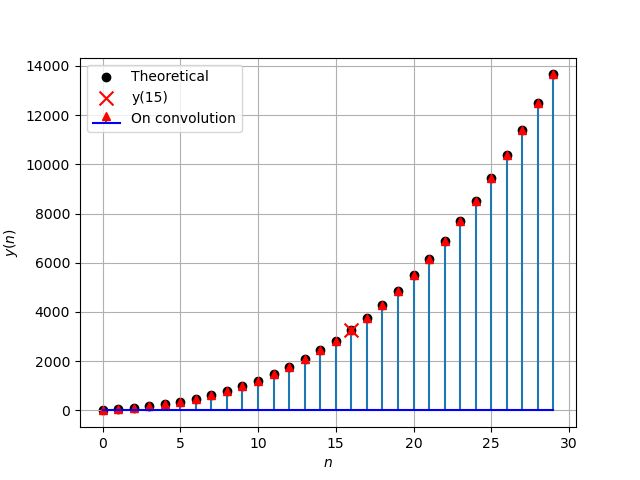
\includegraphics[width=\columnwidth]{ncert-maths/11/9/4/5/figs/plot.png}

\begin{center}
    \caption{Simulation v/s theoretical}
\end{center}
\end{figure}


\newpage

\item Find the sum to indicated number of terms in each of the geometric progressions in
$0.15, 0.015, 0.0015\ldots 20 terms$.\\
\solution
\input{ncert-maths/11/9/3/7/assignment2.tex}
\pagebreak

\item A man deposited Rs 10000 in a bank at the rate of 5\% simple interest anually. Find the amount in 15\textsuperscript{th} year since he deposited the amount and also calculate the total amount after 20 years.\\
\solution
 \iffalse
\let\negmedspace\undefined
\let\negthickspace\undefined
\documentclass[journal,12pt,twocolumn]{IEEEtran}
\usepackage{amssymb}
\usepackage{cite}
\usepackage{amsmath,amssymb,amsfonts,amsthm}
\usepackage{algorithmic}
\usepackage{graphicx}
\usepackage{textcomp}
\usepackage{xcolor}
\usepackage{txfonts}
\usepackage{listings}
\usepackage{enumitem}
\usepackage{mathtools}
\usepackage{gensymb}
\usepackage{comment}
\usepackage[breaklinks=true]{hyperref}
\usepackage{tkz-euclide} 
\usepackage{listings}
\usepackage{gvv}                                        
\def\inputGnumericTable{}                                 
\usepackage[latin1]{inputenc}                                
\usepackage{color}                                            
\usepackage{array}                                            
\usepackage{longtable}                                       
\usepackage{calc}                                             
\usepackage{multirow}                                         
\usepackage{hhline}                                           
\usepackage{ifthen}                                           
\usepackage{lscape}
\usepackage{pgfplots}
\newtheorem{theorem}{Theorem}[section]
\newtheorem{problem}{Problem}
\newtheorem{proposition}{Proposition}[section]
\newtheorem{lemma}{Lemma}[section]
\newtheorem{corollary}[theorem]{Corollary}
\newtheorem{example}{Example}[section]
\newtheorem{definition}[problem]{Definition}
\newcommand{\BEQA}{\begin{eqnarray}}
\newcommand{\EEQA}{\end{eqnarray}}
\newcommand{\define}{\stackrel{\triangle}{=}}
\theoremstyle{remark}
\newtheorem{rem}{Remark}
\begin{document}

\bibliographystyle{IEEEtran}
\vspace{3cm}

\title{NCERT Discrete-11.9.4-5}
\author{EE22BTECH11004 - Allu Lohith}

\maketitle
\newpage
\bigskip


 Find the sum of n terms of this sequence:$$5^2+6^2+7^2...+20^2$$  
\solution
\fi
\begin{table}[h!]
\centering
\renewcommand{\arraystretch}{2}
\begin{tabular}{|c|p{4cm}|c|}
\hline 
\setlength{\tabcolsep}{1pt}
\textbf{Parameter}  &\textbf{Description} &\textbf{Formulae/Value} \\
\hline
n & Iteration number starting from zero till 15 & - \\
\hline
$x\brak n$ & General term of the sequence from $n=0$ to $n=15$ &$\brak{n+5}^2$  u\brak n\\
\hline
$x\brak 0$ & First term of the sequence & 5 \\
\hline
\end{tabular}

\vspace{0.5cm}
\caption{\normalsize Parameters}
\end{table}
The standard $z$ transforms,
\begin{align}
    u \brak n &\stackrel{z}{\longleftrightarrow} \frac{1}{1-z^{-1}}, \abs z >1\\
   n u\brak n &\stackrel{z}{\longleftrightarrow} \frac{z^{-1}}{\brak{1-z^{-1}}^2}, \abs z >1\\
   n^2 u\brak n &\stackrel{z}{\longleftrightarrow} \frac{z^{-1}\brak{1+z^{-1}}}{\brak{1-z^{-1}}^3}, \abs z >1
\end{align}
As 
\begin{align}
    x\brak n = \brak{n^2+10n+25}u\brak n
\end{align}
The $z$ transform of general term can be written as , 
\begin{align}
    X\brak z &= \frac{z^{-1}\brak{1+z^{-1}}}{\brak{1-z^{-1}}^3}+10\frac{z^{-1}}{\brak{1-z^{-1}}^2}+\frac{25}{1-z^{-1}} \\
    X\brak z &=  \frac{16z^{-2}-39z^{-1}+25}{\brak{1-z^{-1}}^3}; \abs{z}>1
\end{align}
On convolution for finding the sum
\begin{align}
    y\brak n= x\brak n \ast u\brak n
\end{align}
On z transform,
\begin{align}
    Y\brak z &= X \brak z \cdot U \brak z\\
    &= \brak{\frac{16z^{-2}-39z^{-1}+25}{\brak{1-z^{-1}})^3}} \cdot \frac{1}{1-z^{-1}}\\
    \implies 
    Y \brak z & = \frac{16z^{-2}-39z^{-1}+25}{\brak{1-z^{-1}}^4}; \quad \abs z >1
\end{align}
Using the contour integration to find the inverse $z$ transform,
\begin{align}
    y(n)&=\oint_c Y(z)\cdot z^{n-1}dz\\
    y(21)&=\oint_c \brak{\frac{16z^{-2}-39z^{-1}+25}{\brak{1-z^{-1}}^4}} z^{14}dz
\end{align}
As there are four poles from observation, so $m=4$
\begin{align}
    y\brak{21} &= \frac{1}{(m-1)!} \lim_{z \to a} \frac{d^{m-1}}{dz^{m-1}}\brak{(z-a)^mf(z)}\\
    &= \frac{1}{3!} \lim_{z \to 1} \frac{d^{3}}{dz^{3}}\brak{(z-1)^4 \frac{\brak{16z^{-2}-39z^{-1}+25}}{(1-z^{-1})^4} z^{14}}\\
    &= \frac{1}{6} \lim_{z \to 1} \frac{d^{3}}{dz^{3}}\brak{\brak{16z^{-2}-39z^{-1}+25}z^{18}}\\
    &= \frac{1}{6} \lim_{z \to 1} \frac{d^{3}}{dz^{3}}\brak{16z^{16}-39z^{17}+25z^{18}}\\
    &= \frac{1}{6}  \brak{16 \times 18 \times 17 \times 16+14 \times 17 \times 16 \times 15 }\\
    \implies y\brak{21}&=2840 
\end{align}
Hence the sum of the terms of the sequence is 2840.

\begin{figure}[h]
    \centering  

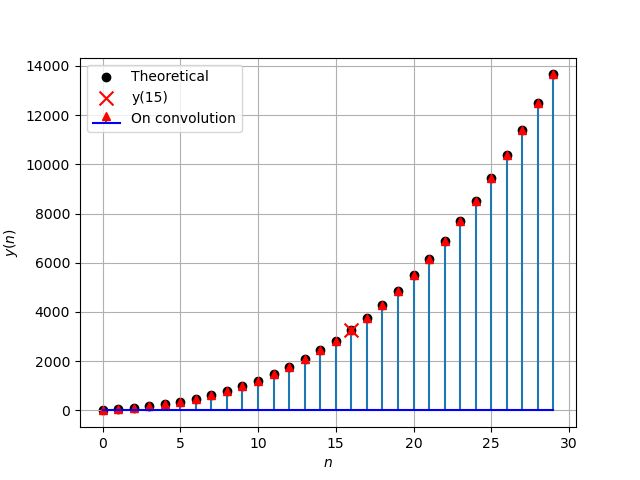
\includegraphics[width=\columnwidth]{ncert-maths/11/9/4/5/figs/plot.png}

\begin{center}
    \caption{Simulation v/s theoretical}
\end{center}
\end{figure}


\pagebreak
\item A manufacturer reckons that the value of a machine, which costs him Rs.$15625$, will depreciate each year by $20\%$.Find the estimated value at the end of 5 years.\\
\solution
 \iffalse
\let\negmedspace\undefined
\let\negthickspace\undefined
\documentclass[journal,12pt,twocolumn]{IEEEtran}
\usepackage{amssymb}
\usepackage{cite}
\usepackage{amsmath,amssymb,amsfonts,amsthm}
\usepackage{algorithmic}
\usepackage{graphicx}
\usepackage{textcomp}
\usepackage{xcolor}
\usepackage{txfonts}
\usepackage{listings}
\usepackage{enumitem}
\usepackage{mathtools}
\usepackage{gensymb}
\usepackage{comment}
\usepackage[breaklinks=true]{hyperref}
\usepackage{tkz-euclide} 
\usepackage{listings}
\usepackage{gvv}                                        
\def\inputGnumericTable{}                                 
\usepackage[latin1]{inputenc}                                
\usepackage{color}                                            
\usepackage{array}                                            
\usepackage{longtable}                                       
\usepackage{calc}                                             
\usepackage{multirow}                                         
\usepackage{hhline}                                           
\usepackage{ifthen}                                           
\usepackage{lscape}
\usepackage{pgfplots}
\newtheorem{theorem}{Theorem}[section]
\newtheorem{problem}{Problem}
\newtheorem{proposition}{Proposition}[section]
\newtheorem{lemma}{Lemma}[section]
\newtheorem{corollary}[theorem]{Corollary}
\newtheorem{example}{Example}[section]
\newtheorem{definition}[problem]{Definition}
\newcommand{\BEQA}{\begin{eqnarray}}
\newcommand{\EEQA}{\end{eqnarray}}
\newcommand{\define}{\stackrel{\triangle}{=}}
\theoremstyle{remark}
\newtheorem{rem}{Remark}
\begin{document}

\bibliographystyle{IEEEtran}
\vspace{3cm}

\title{NCERT Discrete-11.9.4-5}
\author{EE22BTECH11004 - Allu Lohith}

\maketitle
\newpage
\bigskip


 Find the sum of n terms of this sequence:$$5^2+6^2+7^2...+20^2$$  
\solution
\fi
\begin{table}[h!]
\centering
\renewcommand{\arraystretch}{2}
\begin{tabular}{|c|p{4cm}|c|}
\hline 
\setlength{\tabcolsep}{1pt}
\textbf{Parameter}  &\textbf{Description} &\textbf{Formulae/Value} \\
\hline
n & Iteration number starting from zero till 15 & - \\
\hline
$x\brak n$ & General term of the sequence from $n=0$ to $n=15$ &$\brak{n+5}^2$  u\brak n\\
\hline
$x\brak 0$ & First term of the sequence & 5 \\
\hline
\end{tabular}

\vspace{0.5cm}
\caption{\normalsize Parameters}
\end{table}
The standard $z$ transforms,
\begin{align}
    u \brak n &\stackrel{z}{\longleftrightarrow} \frac{1}{1-z^{-1}}, \abs z >1\\
   n u\brak n &\stackrel{z}{\longleftrightarrow} \frac{z^{-1}}{\brak{1-z^{-1}}^2}, \abs z >1\\
   n^2 u\brak n &\stackrel{z}{\longleftrightarrow} \frac{z^{-1}\brak{1+z^{-1}}}{\brak{1-z^{-1}}^3}, \abs z >1
\end{align}
As 
\begin{align}
    x\brak n = \brak{n^2+10n+25}u\brak n
\end{align}
The $z$ transform of general term can be written as , 
\begin{align}
    X\brak z &= \frac{z^{-1}\brak{1+z^{-1}}}{\brak{1-z^{-1}}^3}+10\frac{z^{-1}}{\brak{1-z^{-1}}^2}+\frac{25}{1-z^{-1}} \\
    X\brak z &=  \frac{16z^{-2}-39z^{-1}+25}{\brak{1-z^{-1}}^3}; \abs{z}>1
\end{align}
On convolution for finding the sum
\begin{align}
    y\brak n= x\brak n \ast u\brak n
\end{align}
On z transform,
\begin{align}
    Y\brak z &= X \brak z \cdot U \brak z\\
    &= \brak{\frac{16z^{-2}-39z^{-1}+25}{\brak{1-z^{-1}})^3}} \cdot \frac{1}{1-z^{-1}}\\
    \implies 
    Y \brak z & = \frac{16z^{-2}-39z^{-1}+25}{\brak{1-z^{-1}}^4}; \quad \abs z >1
\end{align}
Using the contour integration to find the inverse $z$ transform,
\begin{align}
    y(n)&=\oint_c Y(z)\cdot z^{n-1}dz\\
    y(21)&=\oint_c \brak{\frac{16z^{-2}-39z^{-1}+25}{\brak{1-z^{-1}}^4}} z^{14}dz
\end{align}
As there are four poles from observation, so $m=4$
\begin{align}
    y\brak{21} &= \frac{1}{(m-1)!} \lim_{z \to a} \frac{d^{m-1}}{dz^{m-1}}\brak{(z-a)^mf(z)}\\
    &= \frac{1}{3!} \lim_{z \to 1} \frac{d^{3}}{dz^{3}}\brak{(z-1)^4 \frac{\brak{16z^{-2}-39z^{-1}+25}}{(1-z^{-1})^4} z^{14}}\\
    &= \frac{1}{6} \lim_{z \to 1} \frac{d^{3}}{dz^{3}}\brak{\brak{16z^{-2}-39z^{-1}+25}z^{18}}\\
    &= \frac{1}{6} \lim_{z \to 1} \frac{d^{3}}{dz^{3}}\brak{16z^{16}-39z^{17}+25z^{18}}\\
    &= \frac{1}{6}  \brak{16 \times 18 \times 17 \times 16+14 \times 17 \times 16 \times 15 }\\
    \implies y\brak{21}&=2840 
\end{align}
Hence the sum of the terms of the sequence is 2840.

\begin{figure}[h]
    \centering  

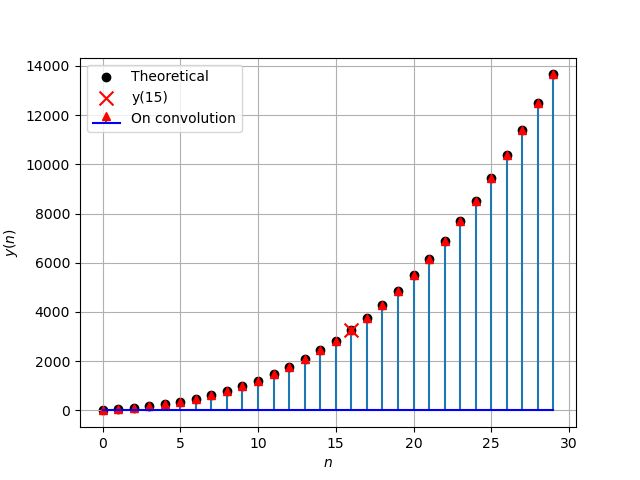
\includegraphics[width=\columnwidth]{ncert-maths/11/9/4/5/figs/plot.png}

\begin{center}
    \caption{Simulation v/s theoretical}
\end{center}
\end{figure}


\pagebreak


\item The houses of a row are numbered consecutively from 1 to 49. Show that there is a value
of x such that the sum of the numbers of the houses preceding the house numbered is equal to the sum of the numbers of the houses following it. Find this value of $x$.\\
Hint:$ S_{x-1}=S_{49}-S_x$\\
\solution
\input{ncert-maths/10/5/4/4/discrete.tex}
\pagebreak

\item A contract on construction job specifies a penalty for delay of completion beyond a certain date as follows: \rupee $200$ for the first day, \rupee $250$ for the second day, \rupee $300$ for the third day, etc., the penalty for each succeeding day being \rupee $50$ more than for the preceding day.How much money the contractor has to pay as penalty, if he has delayed the work by $30$ days?\\
\solution
\input{ncert-maths/10/5/3/15/assign10_5_3_15.tex}
\item Find the sum of all two digit numbers which when divided by $4$,yields $1$ as reminder?\\
\solution
\input{ncert-maths/11/9/5/6/discrete1.tex}
\pagebreak

\item A spiral is made up of successive semicircles,with centres alternately at A and B,starting with centre at A,of radii $0.5cm,1.0cm,1.5cm,2.0cm$,... as shown in Fig.$5.4$.what is the total length of such a spiral made up of thirteen consecutive semicircles?(Take $\pi=\frac{22}{7}$)\\
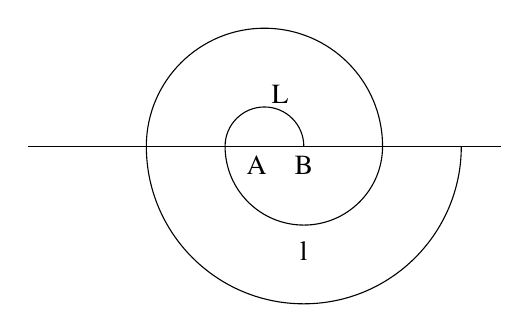
\begin{tikzpicture}

% Define the centers A and B
\coordinate (A) at (0,0);
\coordinate (B) at (0.5,0);

% Draw the spiral using semicircles
\foreach \r in {0.5,1.5} {
  \draw (A) ++(\r,0) arc (0:180:\r);
}
\foreach \r in {1.0,2.0} {
  \draw (B) ++(\r,0) arc (0:-180:\r);
}
\node[label={above:A}] at (-0.1,-0.6){};
\node[label={above:B}] at (0.5,-0.6){};
\node[label={above:l}] at (0.5,-1.7){};
\node[label={above:L}] at (0.2,0.3){};
% Draw the axes (optional)
\draw[-] (-3,0) -- (3,0);

\end{tikzpicture}\\
\solution
\pagebreak
\item Evaluate $\sum_{k=1}^{11} (2 + 3^k)$\\
\solution
\pagebreak

\item 200 logs are stacked in the following manner: 20 logs in the bottom row, 19 in the next row,18 in the row next to it and so on (see Fig \ref{fig:10.5.3.19.q}). In how many rows are the 200 logs placed and how many logs are in the top row?
\begin{figure}[h]
    \centering
    \includegraphics[width=1\linewidth]{ncert-maths/10/5/3/19/figs/question.png}
    \caption{ }
    \label{fig:10.5.3.19.q}
\end{figure}
\solution \input{ncert-maths/10/5/3/19/assign2.tex}
\pagebreak

\item In an AP:
\begin{enumerate}
\item given a = 5, d = 3,$a_n=5$, find n and $S_n$.
\item given a = 7, $a_{13}$=35, find d and $S_{13}$.
\item given $a_{12}=37$, d = 3, find a and $S_{12}$.
\item given $a_3$= 15, $S_{10}$ = 125, find d and $a_{10}$.
\item given d = 5, $S_9$= 75, find a and $a_9$.
\item given a = 2, d = 8, $S_n$= 90, find n and $a_n$.
\item given a = 8, $a_n$= 62, $S_n$= 210, find n and d.
\item given an= 4, d = 2, $S_n=-14$, find n and a.
\item given a = 3, n = 8, S = 192, find d.
\item given l = 28, S = 144, and there are total 9 terms. Find a.\\
\end{enumerate}
\solution
\pagebreak

\item Find the sum of n terms of the series:
$1\times2+2\times3+3\times4+4\times5+....$\\
\solution
\pagebreak
\item Find the sum of the first 22 terms of an AP in which $d = 7$ and the $22^{nd}$ term is 149.\\
\solution
\iffalse
\let\negmedspace\undefined
\let\negthickspace\undefined
\documentclass[journal,12pt,twocolumn]{IEEEtran}
\usepackage{amssymb}
\usepackage{cite}
\usepackage{amsmath,amssymb,amsfonts,amsthm}
\usepackage{algorithmic}
\usepackage{graphicx}
\usepackage{textcomp}
\usepackage{xcolor}
\usepackage{txfonts}
\usepackage{listings}
\usepackage{enumitem}
\usepackage{mathtools}
\usepackage{gensymb}
\usepackage{comment}
\usepackage[breaklinks=true]{hyperref}
\usepackage{tkz-euclide} 
\usepackage{listings}
\usepackage{gvv}                                        
\def\inputGnumericTable{}                                 
\usepackage[latin1]{inputenc}                                
\usepackage{color}                                            
\usepackage{array}                                            
\usepackage{longtable}                                       
\usepackage{calc}                                             
\usepackage{multirow}                                         
\usepackage{hhline}                                           
\usepackage{ifthen}                                           
\usepackage{lscape}
\usepackage{pgfplots}
\newtheorem{theorem}{Theorem}[section]
\newtheorem{problem}{Problem}
\newtheorem{proposition}{Proposition}[section]
\newtheorem{lemma}{Lemma}[section]
\newtheorem{corollary}[theorem]{Corollary}
\newtheorem{example}{Example}[section]
\newtheorem{definition}[problem]{Definition}
\newcommand{\BEQA}{\begin{eqnarray}}
\newcommand{\EEQA}{\end{eqnarray}}
\newcommand{\define}{\stackrel{\triangle}{=}}
\theoremstyle{remark}
\newtheorem{rem}{Remark}
\begin{document}

\bibliographystyle{IEEEtran}
\vspace{3cm}

\title{NCERT Discrete-10.5.3-7}
\author{EE22BTECH11004 - Allu Lohith}

\maketitle
\newpage
\bigskip

\renewcommand{\thefigure}{\theenumi}
\renewcommand{\thetable}{\theenumi}
Find the sum of the first 22 terms of an AP in which $d = 7$ and the 22nd term is 149.\\

\solution
\fi
\begin{table}[h!]
\centering
\renewcommand{\arraystretch}{2}
\begin{tabular}{|c|c|c|}
\hline 
\setlength{\tabcolsep}{1pt}
\textbf{Parameter}  &\textbf{Description} &\textbf{Formulae/Value} \\
\hline
$u\brak n$ & Unit step function & $\begin{cases}
0, & \text{if } n < 0, \\
1, & \text{if } n \geq 0.
\end{cases}$\\
\hline
$x\brak 0$ & First term of A.P & - \\
\hline
\textbf{$d$} & Commom difference & 7 \\
\hline
n & Count of terms starting from '0' & - \\
\hline
$x\brak n$ & $(n+1)^{th}$ term of the A.P & $\brak{x(0)+nd}u\brak n$ \\
\hline
$x\brak{21}$ & Value of $22^{nd}$ term & 149 \\

\hline

\end{tabular}

\vspace{0.5cm}
\caption{\normalsize Parameters}
\end{table}

Now, the $22^{nd}$ term means $x(21)$, so

\begin{align}
x(21) &= \brak{x(0)+nd}u\brak {21}\\
149 &= \brak{x(0)+21\brak 7}\brak 1\\
x(0) &= 2    
\end{align}
The standard $z$ transforms,
\begin{align}
    u \brak n &\stackrel{z}{\longleftrightarrow} \frac{1}{1-z^{-1}}, \abs z >1\\
   n u\brak n &\stackrel{z}{\longleftrightarrow} \frac{z^{-1}}{\brak{1-z^{-1}}^2}, \abs z >1
\end{align}
The general term is $x(n)=\brak {2+7n}u\brak n$,
The $z$ transform of the general term is 
\begin{align}
X(z)&= \frac{x(0)}{1-z^{-1}}+\frac{dz^{-1}}{\brak{1-z^{-1}}^2} \\
&=\frac{2}{1-z^{-1}}+\frac{7z^{-1}}{{\brak{1-z^{-1}}^2}}\\
&=\frac{2+5z^{-1}}{\brak{1-z^{-1}}^2} ; \quad \abs z>1
\end{align}
On convolution for finding the sum
\begin{align}
    y(n)=x(n)\ast u(n)
\end{align}
On z-transform, 
\begin{align}
Y(z)&=X(z)\cdot U(z)\\
    &=\brak{\frac{{2+5z^{-1}}}{{(1-z^{-1})^2}}} \cdot \frac{1}{{1-z^{-1}}}\\
  \implies Y(z)  &= \frac{2+5z^{-1}}{\brak{1-z^{-1}}^3} ; \quad \quad \abs z>1
\end{align}
Using Contour integration to find the inverse z-transform,
\begin{align}
    y(n)&=\oint_c Y(z)\cdot z^{n-1}dz\\
    y(21)&=\oint_c \frac{2+5z^{-1}}{\brak{1-z^{-1}}^3}\cdot z^{20}dz
\end{align}
We can observe there are three poles and thus m = 3,
\begin{align}
    y\brak{21}&=\frac{1}{\brak{m-1}!} \lim_{z \to a} \frac{d^{m-1}}{dz^{m-1}}\brak{\brak{z-a}^mf\brak z}\\
    &=\frac{1}{2!}\lim_{z \to 1} \frac{d^2}{dz^2} \brak{\brak{z-1}^3\cdot \frac{2+5z^{-1}}{\brak{1-z^{-1}}^3}\cdot \brak{z^{20}}}\\
    &=\frac{1}{2}\brak{1012+2310}\\
    \implies y \brak{21}&=1661
\end{align}
\begin{figure}[h]
    \centering  

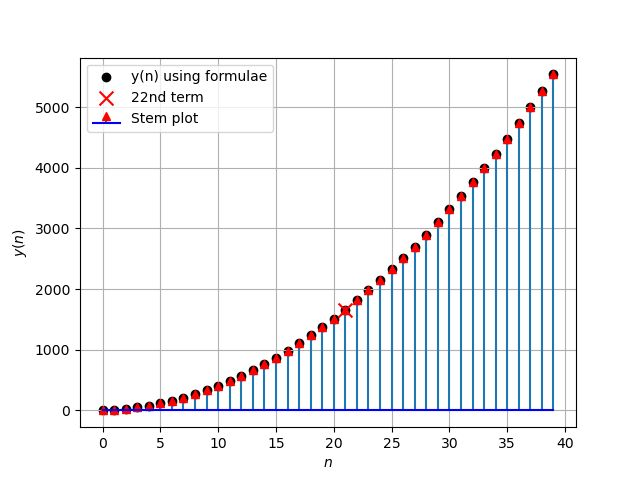
\includegraphics[width=\columnwidth]{ncert-maths/10/5/3/7/figs/plot.png}

\begin{center}
    \caption{Simulation v/s theoretical}
\end{center}
\end{figure}


\pagebreak

\item Find the sum of integers from 1 to 100 that are divisible by 2 or 5.\\
\solution
\pagebreak

\item In a school, students thought of planting trees in and around the school to reduce air

pollution. It was decided that the number of trees, that each section of each class will

plant, will be the same as the class, in which they are studying, e.g., a section of Class I

will plant 1 tree, a section of Class II will plant 2 trees and so on till Class XII. There are

three sections of each class. How many trees will be planted by the students?\\
\solution
\pagebreak
\item A sum of Rs.$700$ is to be used to give seven cash prizes to students of a school for their overall academic performance. If each prize is Rs.$20$ less than its preceding prize, find the value of each of the prizes. \\
\solution
\input{ncert-maths/10/5/3/16/Ncert_10_5_3_16.tex}
\pagebreak

\item Find the sum of all numbers between 200 and 400 which are divisible by 7.\\
\solution
 \iffalse
\let\negmedspace\undefined
\let\negthickspace\undefined
\documentclass[journal,12pt,twocolumn]{IEEEtran}
\usepackage{amssymb}
\usepackage{cite}
\usepackage{amsmath,amssymb,amsfonts,amsthm}
\usepackage{algorithmic}
\usepackage{graphicx}
\usepackage{textcomp}
\usepackage{xcolor}
\usepackage{txfonts}
\usepackage{listings}
\usepackage{enumitem}
\usepackage{mathtools}
\usepackage{gensymb}
\usepackage{comment}
\usepackage[breaklinks=true]{hyperref}
\usepackage{tkz-euclide} 
\usepackage{listings}
\usepackage{gvv}                                        
\def\inputGnumericTable{}                                 
\usepackage[latin1]{inputenc}                                
\usepackage{color}                                            
\usepackage{array}                                            
\usepackage{longtable}                                       
\usepackage{calc}                                             
\usepackage{multirow}                                         
\usepackage{hhline}                                           
\usepackage{ifthen}                                           
\usepackage{lscape}
\usepackage{pgfplots}
\newtheorem{theorem}{Theorem}[section]
\newtheorem{problem}{Problem}
\newtheorem{proposition}{Proposition}[section]
\newtheorem{lemma}{Lemma}[section]
\newtheorem{corollary}[theorem]{Corollary}
\newtheorem{example}{Example}[section]
\newtheorem{definition}[problem]{Definition}
\newcommand{\BEQA}{\begin{eqnarray}}
\newcommand{\EEQA}{\end{eqnarray}}
\newcommand{\define}{\stackrel{\triangle}{=}}
\theoremstyle{remark}
\newtheorem{rem}{Remark}
\begin{document}

\bibliographystyle{IEEEtran}
\vspace{3cm}

\title{NCERT Discrete-11.9.4-5}
\author{EE22BTECH11004 - Allu Lohith}

\maketitle
\newpage
\bigskip


 Find the sum of n terms of this sequence:$$5^2+6^2+7^2...+20^2$$  
\solution
\fi
\begin{table}[h!]
\centering
\renewcommand{\arraystretch}{2}
\begin{tabular}{|c|p{4cm}|c|}
\hline 
\setlength{\tabcolsep}{1pt}
\textbf{Parameter}  &\textbf{Description} &\textbf{Formulae/Value} \\
\hline
n & Iteration number starting from zero till 15 & - \\
\hline
$x\brak n$ & General term of the sequence from $n=0$ to $n=15$ &$\brak{n+5}^2$  u\brak n\\
\hline
$x\brak 0$ & First term of the sequence & 5 \\
\hline
\end{tabular}

\vspace{0.5cm}
\caption{\normalsize Parameters}
\end{table}
The standard $z$ transforms,
\begin{align}
    u \brak n &\stackrel{z}{\longleftrightarrow} \frac{1}{1-z^{-1}}, \abs z >1\\
   n u\brak n &\stackrel{z}{\longleftrightarrow} \frac{z^{-1}}{\brak{1-z^{-1}}^2}, \abs z >1\\
   n^2 u\brak n &\stackrel{z}{\longleftrightarrow} \frac{z^{-1}\brak{1+z^{-1}}}{\brak{1-z^{-1}}^3}, \abs z >1
\end{align}
As 
\begin{align}
    x\brak n = \brak{n^2+10n+25}u\brak n
\end{align}
The $z$ transform of general term can be written as , 
\begin{align}
    X\brak z &= \frac{z^{-1}\brak{1+z^{-1}}}{\brak{1-z^{-1}}^3}+10\frac{z^{-1}}{\brak{1-z^{-1}}^2}+\frac{25}{1-z^{-1}} \\
    X\brak z &=  \frac{16z^{-2}-39z^{-1}+25}{\brak{1-z^{-1}}^3}; \abs{z}>1
\end{align}
On convolution for finding the sum
\begin{align}
    y\brak n= x\brak n \ast u\brak n
\end{align}
On z transform,
\begin{align}
    Y\brak z &= X \brak z \cdot U \brak z\\
    &= \brak{\frac{16z^{-2}-39z^{-1}+25}{\brak{1-z^{-1}})^3}} \cdot \frac{1}{1-z^{-1}}\\
    \implies 
    Y \brak z & = \frac{16z^{-2}-39z^{-1}+25}{\brak{1-z^{-1}}^4}; \quad \abs z >1
\end{align}
Using the contour integration to find the inverse $z$ transform,
\begin{align}
    y(n)&=\oint_c Y(z)\cdot z^{n-1}dz\\
    y(21)&=\oint_c \brak{\frac{16z^{-2}-39z^{-1}+25}{\brak{1-z^{-1}}^4}} z^{14}dz
\end{align}
As there are four poles from observation, so $m=4$
\begin{align}
    y\brak{21} &= \frac{1}{(m-1)!} \lim_{z \to a} \frac{d^{m-1}}{dz^{m-1}}\brak{(z-a)^mf(z)}\\
    &= \frac{1}{3!} \lim_{z \to 1} \frac{d^{3}}{dz^{3}}\brak{(z-1)^4 \frac{\brak{16z^{-2}-39z^{-1}+25}}{(1-z^{-1})^4} z^{14}}\\
    &= \frac{1}{6} \lim_{z \to 1} \frac{d^{3}}{dz^{3}}\brak{\brak{16z^{-2}-39z^{-1}+25}z^{18}}\\
    &= \frac{1}{6} \lim_{z \to 1} \frac{d^{3}}{dz^{3}}\brak{16z^{16}-39z^{17}+25z^{18}}\\
    &= \frac{1}{6}  \brak{16 \times 18 \times 17 \times 16+14 \times 17 \times 16 \times 15 }\\
    \implies y\brak{21}&=2840 
\end{align}
Hence the sum of the terms of the sequence is 2840.

\begin{figure}[h]
    \centering  

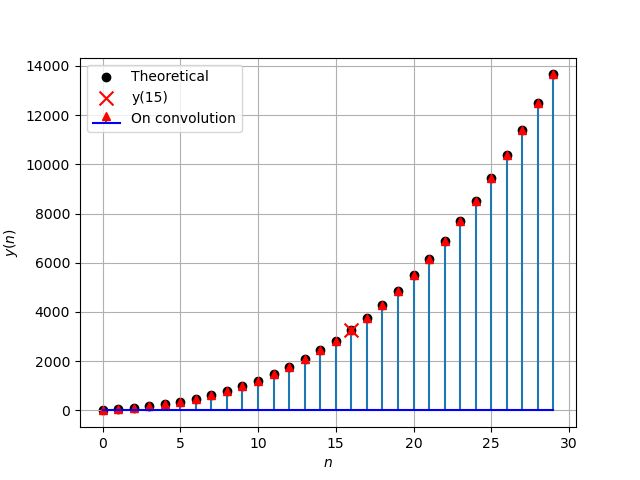
\includegraphics[width=\columnwidth]{ncert-maths/11/9/4/5/figs/plot.png}

\begin{center}
    \caption{Simulation v/s theoretical}
\end{center}
\end{figure}


\pagebreak

\item Find the 20th term in this series.\\
$$2\times4+4\times6+6\times8\cdots+n\,terms$$ \\
\solution 
\input{ncert-maths/11/9/5/22/digital2.tex}
\pagebreak

\item Find the sum of the following APs:
\begin{enumerate}[label=(\alph*)]
\item $2, 7, 12, \ldots$ to $10$ terms.
\item $-37, -33, -29, \ldots$ to $12$ terms.
\item $0.6, 1.7, 2.8, \ldots$ to $100$ terms.
\item $\frac{1}{15}, \frac{1}{12}, \frac{1}{10}, \ldots$ to $11$ terms.
\end{enumerate}
\solution
 \iffalse
\let\negmedspace\undefined
\let\negthickspace\undefined
\documentclass[journal,12pt,twocolumn]{IEEEtran}
\usepackage{amssymb}
\usepackage{cite}
\usepackage{amsmath,amssymb,amsfonts,amsthm}
\usepackage{algorithmic}
\usepackage{graphicx}
\usepackage{textcomp}
\usepackage{xcolor}
\usepackage{txfonts}
\usepackage{listings}
\usepackage{enumitem}
\usepackage{mathtools}
\usepackage{gensymb}
\usepackage{comment}
\usepackage[breaklinks=true]{hyperref}
\usepackage{tkz-euclide} 
\usepackage{listings}
\usepackage{gvv}                                        
\def\inputGnumericTable{}                                 
\usepackage[latin1]{inputenc}                                
\usepackage{color}                                            
\usepackage{array}                                            
\usepackage{longtable}                                       
\usepackage{calc}                                             
\usepackage{multirow}                                         
\usepackage{hhline}                                           
\usepackage{ifthen}                                           
\usepackage{lscape}
\usepackage{pgfplots}
\newtheorem{theorem}{Theorem}[section]
\newtheorem{problem}{Problem}
\newtheorem{proposition}{Proposition}[section]
\newtheorem{lemma}{Lemma}[section]
\newtheorem{corollary}[theorem]{Corollary}
\newtheorem{example}{Example}[section]
\newtheorem{definition}[problem]{Definition}
\newcommand{\BEQA}{\begin{eqnarray}}
\newcommand{\EEQA}{\end{eqnarray}}
\newcommand{\define}{\stackrel{\triangle}{=}}
\theoremstyle{remark}
\newtheorem{rem}{Remark}
\begin{document}

\bibliographystyle{IEEEtran}
\vspace{3cm}

\title{NCERT Discrete-11.9.4-5}
\author{EE22BTECH11004 - Allu Lohith}

\maketitle
\newpage
\bigskip


 Find the sum of n terms of this sequence:$$5^2+6^2+7^2...+20^2$$  
\solution
\fi
\begin{table}[h!]
\centering
\renewcommand{\arraystretch}{2}
\begin{tabular}{|c|p{4cm}|c|}
\hline 
\setlength{\tabcolsep}{1pt}
\textbf{Parameter}  &\textbf{Description} &\textbf{Formulae/Value} \\
\hline
n & Iteration number starting from zero till 15 & - \\
\hline
$x\brak n$ & General term of the sequence from $n=0$ to $n=15$ &$\brak{n+5}^2$  u\brak n\\
\hline
$x\brak 0$ & First term of the sequence & 5 \\
\hline
\end{tabular}

\vspace{0.5cm}
\caption{\normalsize Parameters}
\end{table}
The standard $z$ transforms,
\begin{align}
    u \brak n &\stackrel{z}{\longleftrightarrow} \frac{1}{1-z^{-1}}, \abs z >1\\
   n u\brak n &\stackrel{z}{\longleftrightarrow} \frac{z^{-1}}{\brak{1-z^{-1}}^2}, \abs z >1\\
   n^2 u\brak n &\stackrel{z}{\longleftrightarrow} \frac{z^{-1}\brak{1+z^{-1}}}{\brak{1-z^{-1}}^3}, \abs z >1
\end{align}
As 
\begin{align}
    x\brak n = \brak{n^2+10n+25}u\brak n
\end{align}
The $z$ transform of general term can be written as , 
\begin{align}
    X\brak z &= \frac{z^{-1}\brak{1+z^{-1}}}{\brak{1-z^{-1}}^3}+10\frac{z^{-1}}{\brak{1-z^{-1}}^2}+\frac{25}{1-z^{-1}} \\
    X\brak z &=  \frac{16z^{-2}-39z^{-1}+25}{\brak{1-z^{-1}}^3}; \abs{z}>1
\end{align}
On convolution for finding the sum
\begin{align}
    y\brak n= x\brak n \ast u\brak n
\end{align}
On z transform,
\begin{align}
    Y\brak z &= X \brak z \cdot U \brak z\\
    &= \brak{\frac{16z^{-2}-39z^{-1}+25}{\brak{1-z^{-1}})^3}} \cdot \frac{1}{1-z^{-1}}\\
    \implies 
    Y \brak z & = \frac{16z^{-2}-39z^{-1}+25}{\brak{1-z^{-1}}^4}; \quad \abs z >1
\end{align}
Using the contour integration to find the inverse $z$ transform,
\begin{align}
    y(n)&=\oint_c Y(z)\cdot z^{n-1}dz\\
    y(21)&=\oint_c \brak{\frac{16z^{-2}-39z^{-1}+25}{\brak{1-z^{-1}}^4}} z^{14}dz
\end{align}
As there are four poles from observation, so $m=4$
\begin{align}
    y\brak{21} &= \frac{1}{(m-1)!} \lim_{z \to a} \frac{d^{m-1}}{dz^{m-1}}\brak{(z-a)^mf(z)}\\
    &= \frac{1}{3!} \lim_{z \to 1} \frac{d^{3}}{dz^{3}}\brak{(z-1)^4 \frac{\brak{16z^{-2}-39z^{-1}+25}}{(1-z^{-1})^4} z^{14}}\\
    &= \frac{1}{6} \lim_{z \to 1} \frac{d^{3}}{dz^{3}}\brak{\brak{16z^{-2}-39z^{-1}+25}z^{18}}\\
    &= \frac{1}{6} \lim_{z \to 1} \frac{d^{3}}{dz^{3}}\brak{16z^{16}-39z^{17}+25z^{18}}\\
    &= \frac{1}{6}  \brak{16 \times 18 \times 17 \times 16+14 \times 17 \times 16 \times 15 }\\
    \implies y\brak{21}&=2840 
\end{align}
Hence the sum of the terms of the sequence is 2840.

\begin{figure}[h]
    \centering  

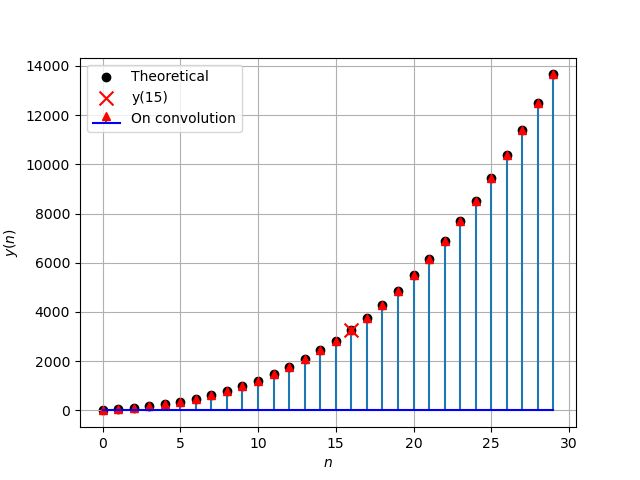
\includegraphics[width=\columnwidth]{ncert-maths/11/9/4/5/figs/plot.png}

\begin{center}
    \caption{Simulation v/s theoretical}
\end{center}
\end{figure}


\pagebreak

\end{enumerate}
